\documentclass{article}
\usepackage{arxiv}
\usepackage[utf8]{inputenc}
\usepackage[T1]{fontenc}
\usepackage{hyperref}
\usepackage{url}
\usepackage{booktabs}
\usepackage{amsfonts}
\usepackage{amsmath}
\usepackage{graphicx}
\usepackage{microtype}
\usepackage{float}
\usepackage[numbers,sort&compress]{natbib}
\graphicspath{{../assets/figures/}}
\renewcommand{\headeright}{Preprint}
\renewcommand{\undertitle}{Preprint}

\title{Sharpening Attention at Inference Recovers Latent\\Length Generalization in Arithmetic Transformers}

\author{
  Micah Bergandi\\
  Independent/Student researcher\\
  \texttt{Micahbergandi@proton.me}
}
\date{}

\begin{document}
\maketitle

\begin{abstract}
Transformers trained on multi-digit addition generalize poorly to operands longer than those seen in training, and the position encodings and input formats that help are known to be sensitive to the random seed. We study this failure on one consumer GPU with models of 3.4M and 11M parameters and report three findings. First, out-of-distribution accuracy is unstable during training: in many runs it peaks between 10k and 25k steps and then declines while in-distribution accuracy remains at 100\%, so that final-checkpoint and best-checkpoint numbers can differ by 50 points. Second, the mechanism these models learn is a ripple-carry adder whose carry is read from the model's own previous output digit, implemented as sharp attention lookups. Third, multiplying the attention logits by a constant at inference, with no retraining, recovers generalization that these lookups lose at longer lengths. An 11M-parameter position-coupling model trained on up to 30-digit operands rises from 0\% to 100\% exact match at 200 digits when its logits are scaled by 2; the intervention acts through the first layer alone. Across 32 runs the intervention helps every model that generalized past its training length at some point and none that did not. Training with the same temperature makes such models more common but does not prevent the decline. Attention-logit scaling has been used as a length-extrapolation heuristic before; our contribution is a controlled setting in which the circuit it acts on can be identified and its effect on a latent computation isolated. Code, checkpoints and all figures are public.
\end{abstract}

\section{Introduction}

A transformer trained to add numbers of up to 20 digits usually cannot add numbers of 25 digits. This length generalization failure has motivated a line of work on input formats and position encodings for arithmetic \citep{lee2023teaching,zhou2024transformers,mcleish2024transformers,cho2024position,aba2025}, with reported generalization factors of 2.5$\times$ to 6$\times$ the training length, and a persistent caveat that the results vary strongly across random seeds \citep{zhou2024transformers}.

This paper began as a reproduction of that literature on a single GPU. Logging out-of-distribution accuracy throughout training, rather than at the end, showed that it often rises early and then declines while training and in-distribution accuracy stay at 100\%. Locating the carry mechanism in a model that had generalized showed that it consists of two sharp attention lookups. Together these suggested that the failure at longer lengths, and the decline during training, might be failures of attention contrast rather than of the algorithm, and that sharpening attention at inference should help models that have the algorithm and not those that do not. That is what we find.

Our contributions are:
\begin{itemize}
  \item A characterization of out-of-distribution accuracy as a transient of training on this task, with ablations showing it is not caused by the learning-rate schedule and is only partly affected by weight decay (Section~\ref{sec:erosion}).
  \item A mechanistic account of the carry in a position-coupling model: a ripple-carry adder that reads the incoming carry from the model's previous output digit, verified by counterfactual interventions and shown to handle carry chains of any length (Section~\ref{sec:carry}).
  \item An inference-time intervention, scaling the attention logits by a constant, that takes an 11M-parameter model trained on 30-digit operands from 0\% to 100\% exact match at 200 digits, acts through the first layer alone, and across 32 runs helps exactly the models that generalized at some point during training (Section~\ref{sec:sharpen}).
  \item Evidence that training with the same temperature makes such models more common, stacks with the inference-time intervention, and does not prevent the decline (Section~\ref{sec:training}).
\end{itemize}

Scaling attention logits is not new. \citet{chiang2022overcoming} scale by the logarithm of the sequence length and show this is necessary for self-attention to represent certain formal languages at all lengths; YaRN \citep{peng2023yarn} applies a temperature to attention logits when extending the context window of rotary-position language models. The present setting differs in that the task's algorithm is known, the circuit can be located, the loss of contrast can be measured, and the intervention can be shown to restore a specific latent computation on a per-seed basis.

\section{Related work}

\paragraph{Length generalization in arithmetic.} \citet{lee2023teaching} showed that writing digits least significant first reduces addition to a per-position rule and studied data formats for small transformers. \citet{zhou2024transformers} reached 2.5$\times$ the training length with FIRE position encodings, randomized positions and index hints, and documented large variance across seeds. Abacus embeddings \citep{mcleish2024transformers} restart the position index for each number; position coupling \citep{cho2024position} assigns the same position id to digits of equal significance across operands and answer, and reports 6.7$\times$ generalization. An anonymous ICLR submission \citep{aba2025} inserts aligned blank tokens so that the sequence length is fixed regardless of operand length. We reproduce these methods on a smaller budget and use position coupling for the mechanistic work.

\paragraph{Attention temperature and length.} \citet{chiang2022overcoming} prove that attention with a fixed logit scale cannot represent some formal languages at arbitrary length and that scaling logits by $\log n$ resolves this, with experiments on parity and related tasks. YaRN \citep{peng2023yarn} includes a logit temperature as part of a context-extension recipe. Our intervention is the same operation, applied post hoc as a constant, in a setting where its effect on an identified circuit can be measured.

\paragraph{Grokking.} The project also reproduces the modular-addition grokking results of \citet{power2022grokking} and \citet{nanda2023progress} and the claim of \citet{swaroop2026latent} that Fourier structure precedes generalization, extending the latter to a transformer. Those results are independent of the ones reported here and are documented in the code repository.

\section{Experimental setup}
\label{sec:setup}

\paragraph{Task and format.} The task is addition of two integers with 1 to $N$ digits, presented as the token sequence \texttt{\$a+b=c\$} over a 16-symbol vocabulary. Digits are written least significant first \citep{lee2023teaching}, so answer digit $i$ depends only on the two operand digits in column $i$ and the carry from column $i-1$. Operands are zero-padded to a common length and the answer to one digit more. Examples are generated on the fly. The loss is next-token prediction on the answer tokens and the closing delimiter.

\paragraph{Position schemes.} We compare learned absolute positions, abacus embeddings \citep{mcleish2024transformers} with a random offset during training, position coupling \citep{cho2024position}, and fixed-width aligned blankspace \citep{aba2025}. A learned per-head relative distance bias is included as a control; it is not the relative embedding of \citet{shaw2018self} used in \citet{aba2025}, and we note where this matters.

\paragraph{Models and training.} Pre-norm decoder-only transformers with ReLU MLPs. The small model has 4 layers, width 256 and 4 heads (3.4M parameters) and is trained on operands of 1 to 20 digits for 50k steps with batch size 256. The large model has 6 layers, width 384 and 6 heads (11M parameters) and is trained on 1 to 30 digits for 60k steps with batch size 384. Both use AdamW with cosine decay and weight decay 0.1 unless stated. Each configuration uses three seeds unless stated; the small position-coupling model uses six and the large one four. Full hyperparameters are in Appendix~\ref{app:hyper}.

\paragraph{Evaluation.} Exact match of the full answer under greedy decoding, on 128 to 256 problems whose operands both have exactly $n$ digits, for $n$ up to 100 (small) or 200 (large). All test lengths are evaluated every 2,500 steps during training. Unless stated, we report the final checkpoint.

\section{Out-of-distribution accuracy is a transient of training}
\label{sec:erosion}

Figure~\ref{fig:ladder} shows the final-checkpoint picture for nine input formats on the small model. Formats with sequential positions reach 100\% in distribution and 0\% one digit beyond the training length. Abacus, position coupling and fixed-width blankspace extend past the training length and degrade gradually; none exceeds about 2.5$\times$ on this budget, and the variance across seeds exceeds the differences between methods. Two of six position-coupling seeds generalize at all.

\begin{figure}[t]
\centering
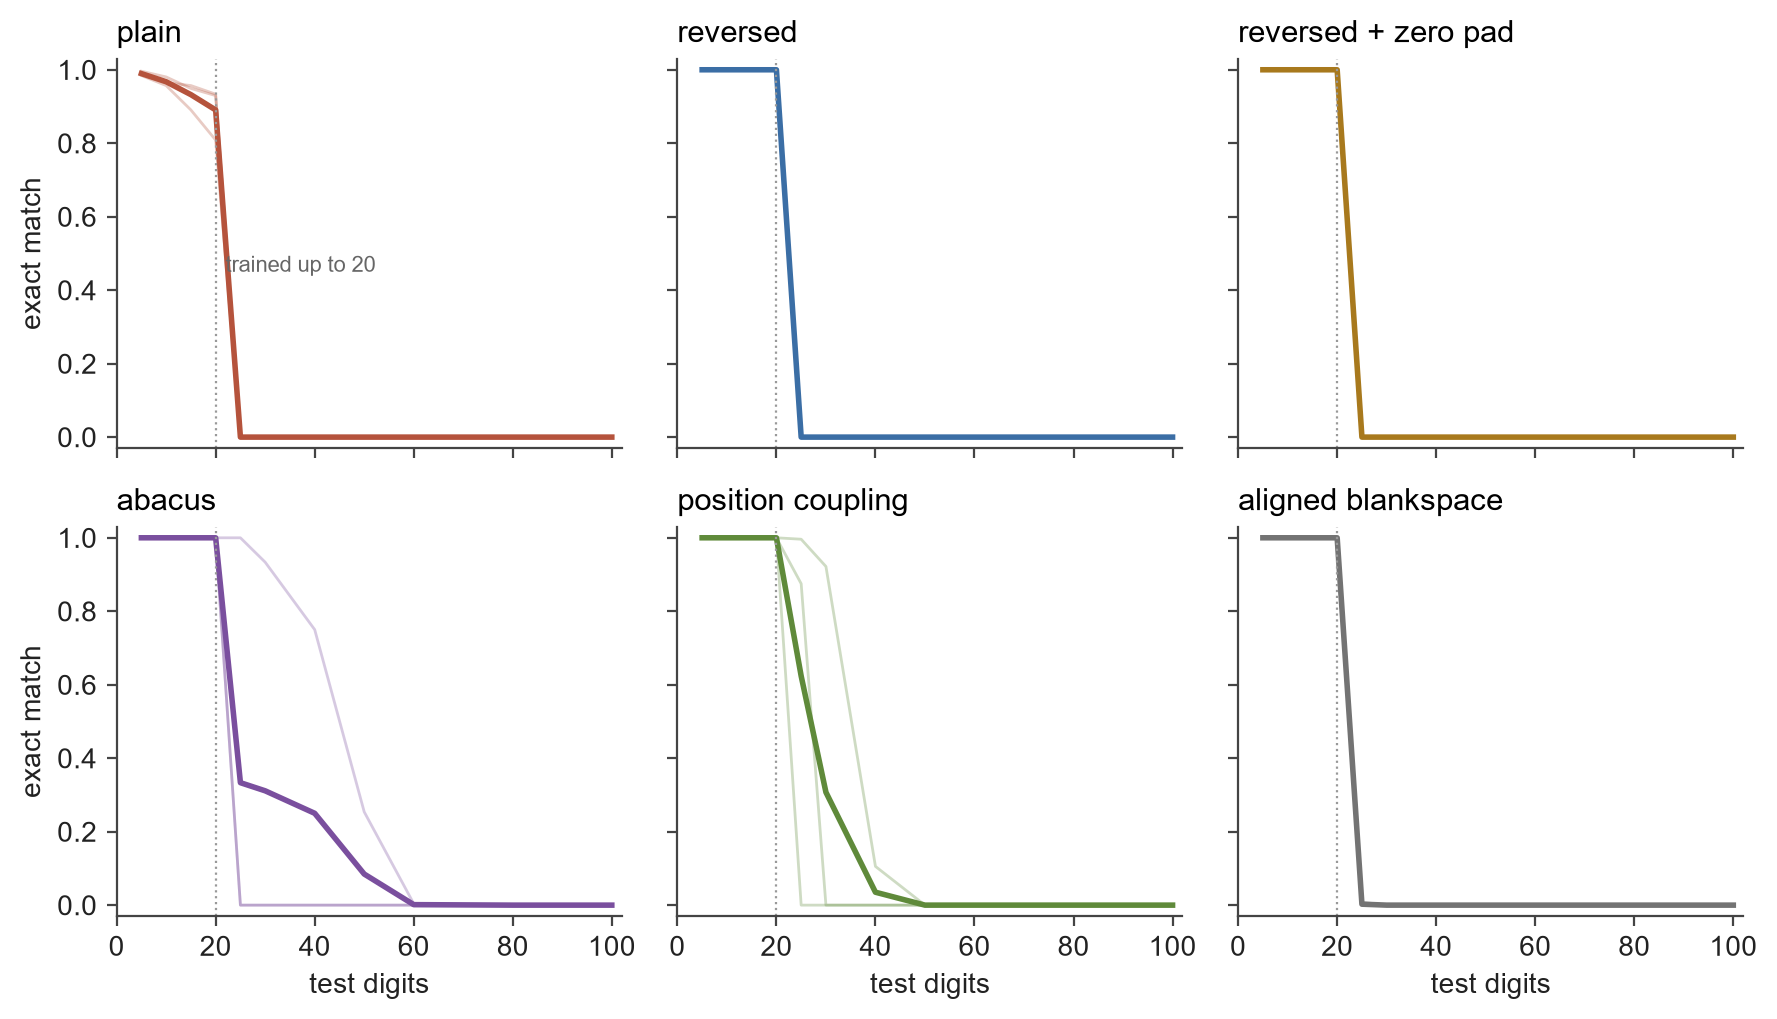
\includegraphics[width=\linewidth]{length_ladder.png}
\caption{Exact match versus test length for nine input formats on the 3.4M model trained on 1 to 20 digits (dotted line). Faint lines are individual seeds; bold is the mean. The blankspace variants follow \citet{aba2025}. The relative-position rows use a per-head distance bias rather than the relative embeddings of that paper, and its headline combination did not train under this substitution.}
\label{fig:ladder}
\end{figure}

Figure~\ref{fig:erosion} shows the same quantity during training. In every run that generalized, out-of-distribution accuracy rose, peaked between 10k and 25k steps, and declined, while accuracy at the training length stayed at 100\% and the training loss continued to decrease. The best small seed reached 63\% at 40 digits at step 17k and finished at 11\%. One large seed reached 85\% at 60 digits at step 15k and finished at 75\%.

\begin{figure}[t]
\centering
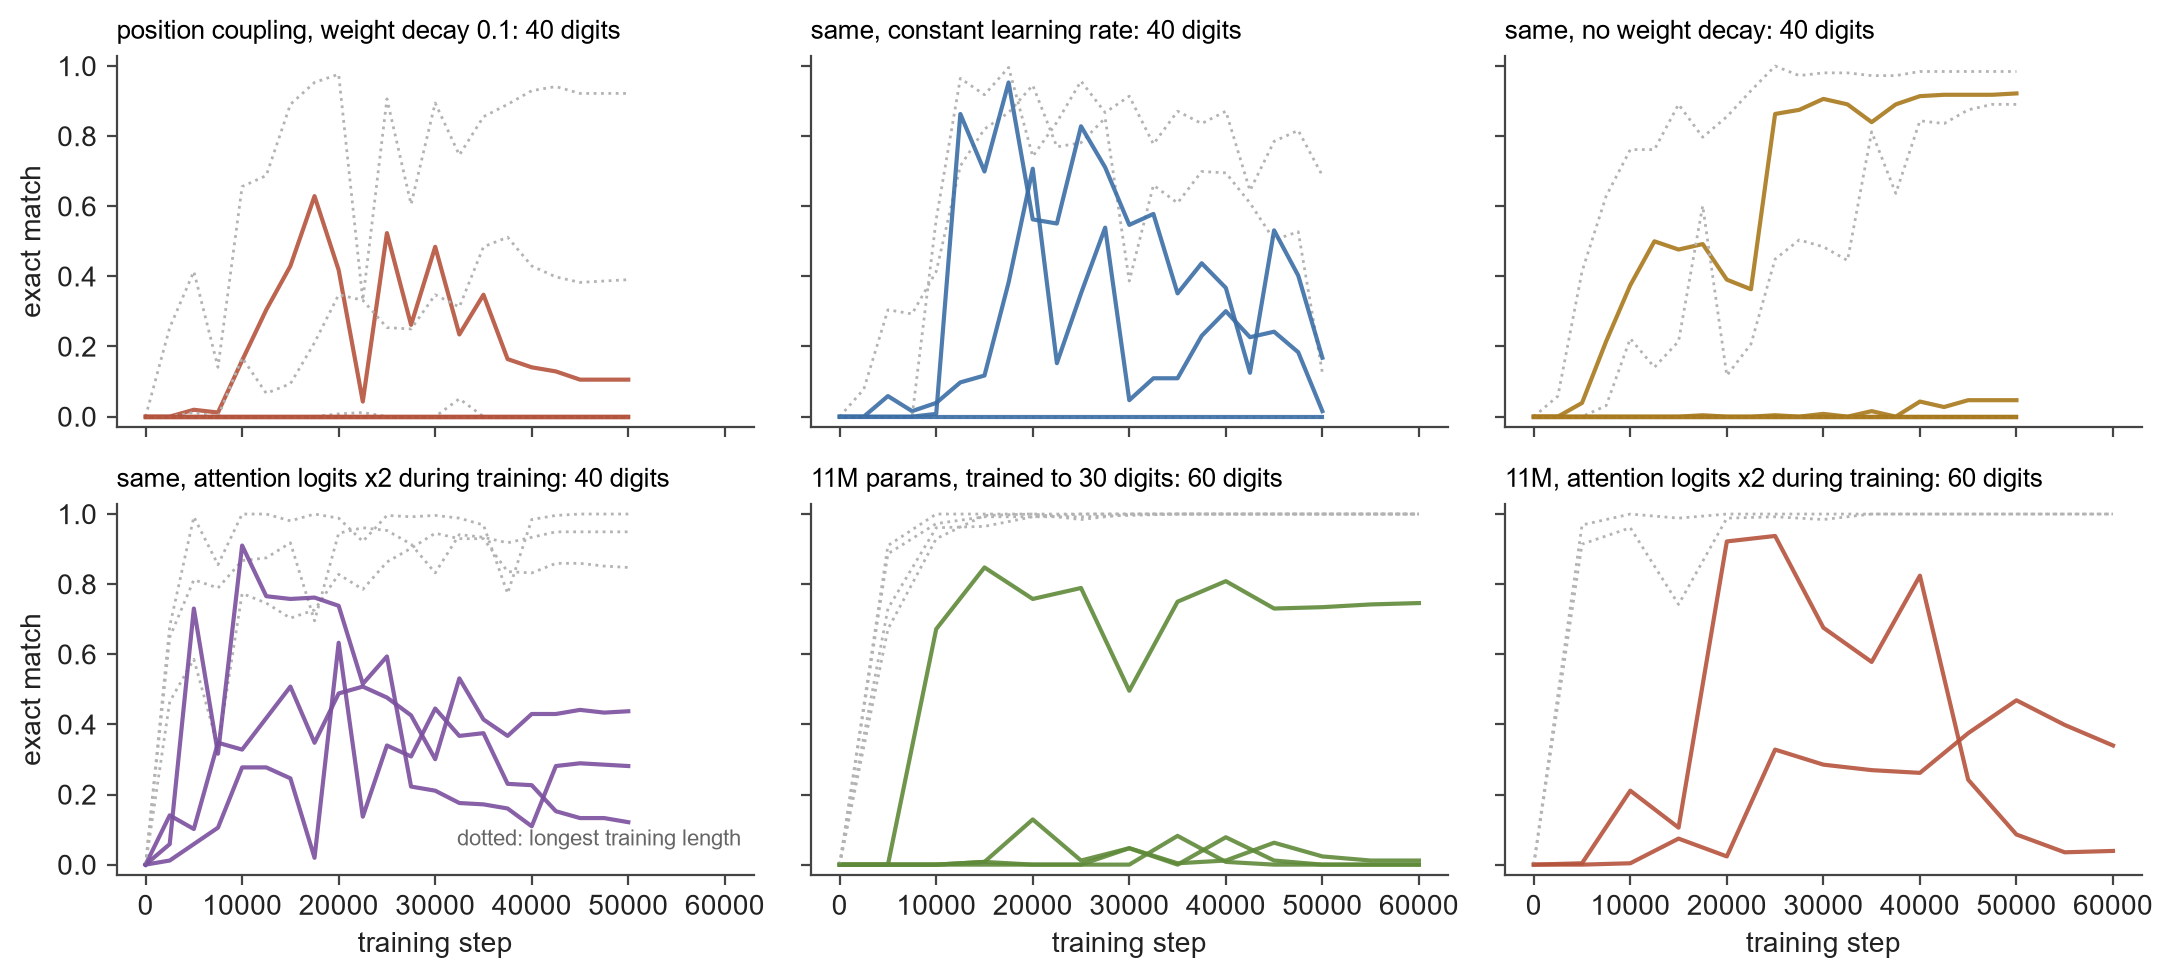
\includegraphics[width=\linewidth]{generalization_over_training.png}
\caption{Out-of-distribution exact match during training for position-coupling runs, one line per seed, at a fixed length beyond the training length (40 digits for the 3.4M model, 60 for the 11M model). Dotted lines: accuracy at the longest training length. Bottom left and bottom right: models trained with attention logits scaled by 2 (Section~\ref{sec:training}).}
\label{fig:erosion}
\end{figure}

Two ablations on the small model rule out the obvious causes. With a constant learning rate instead of cosine decay the decline is larger (one seed from 71\% to 2\%), so the schedule is not responsible; if anything, the decay to zero freezes the model in whatever state it has reached. Without weight decay, the two of six seeds that generalized improved monotonically and kept their accuracy, but the fraction of seeds that generalized was unchanged. Weight decay therefore contributes in some runs but does not determine the outcome. Independently of the cause, the measurement consequence stands: for these methods, the final checkpoint and the best checkpoint can differ by 50 points of exact match, and results reported at one are not comparable with results reported at the other.

\section{The carry circuit}
\label{sec:carry}

We take the best small position-coupling model and ask how it computes the carry when predicting answer digit $i$. Three measurements are shown in Figure~\ref{fig:carry}: attention mass at the predicting position by source (the two digits of column $i$, the two digits of column $i-1$, the model's previous output digit $c_{i-1}$, delimiters, or other digits); teacher-forced accuracy on digit $i$ when the carry into column $i$ originated $k$ columns below and propagated through $k$ columns summing to exactly 9; and a counterfactual in which $c_{i-1}$ in the prefix is replaced by the digit it would have been without its incoming carry.

\begin{figure}[t]
\centering
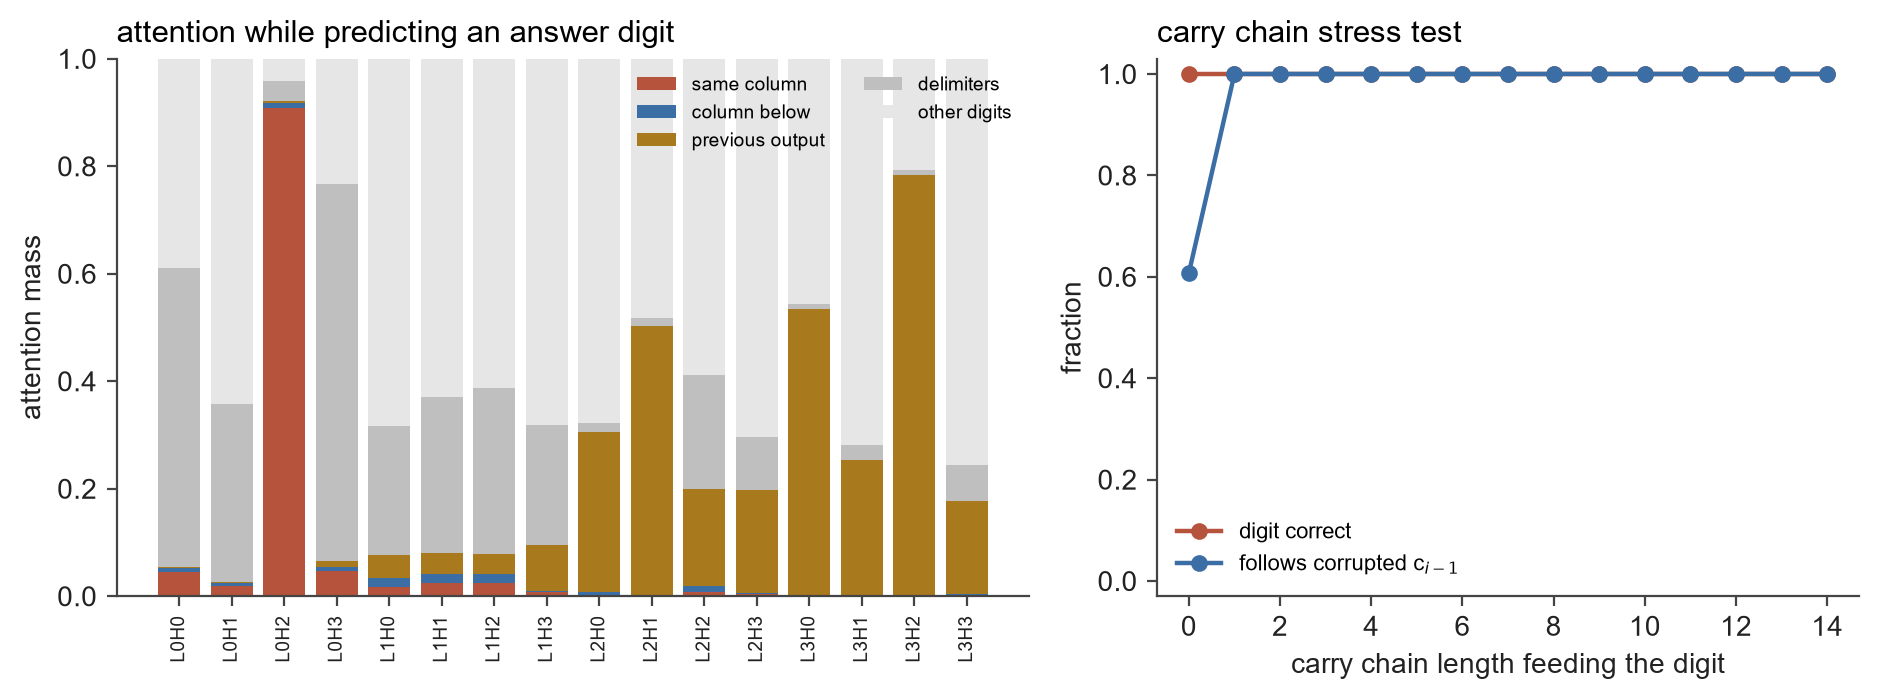
\includegraphics[width=\linewidth]{find_the_carry.png}
\caption{Left: attention by source at the position that predicts an answer digit, per head, averaged over answer positions and 512 problems. Right: teacher-forced accuracy on the digit at the top of a carry chain, versus chain length, and the fraction of predictions that follow a corrupted previous output digit.}
\label{fig:carry}
\end{figure}

The circuit is a ripple-carry adder whose carry is transmitted through the output sequence. One head in layer 0 places 91\% of its attention on the two digits of the current column. Heads in layers 2 and 3 attend to the previous output digit. Whenever column $i-1$ sums to 9, so that the carry into column $i$ depends on the carry into column $i-1$, corrupting $c_{i-1}$ changes the prediction for $c_i$ in 100\% of cases, for every chain length tested. The model reads its own last digit, compares it with $a_{i-1}+b_{i-1}$, and infers whether a carry arrived. Because the recursion runs through autoregressive decoding rather than through depth, chain length has no cost: teacher-forced accuracy is 100\% for chains up to 14 columns. Each step of the circuit is an attention lookup of one or two tokens.

\section{Sharpening attention at inference}
\label{sec:sharpen}

\subsection{Dilution with length}

If the circuit consists of sharp lookups, a longer sequence, in which more tokens share each coupled position id, should dilute them. Figure~\ref{fig:dilution} (left) shows that the digit-adder head's attention mass on its own column decreases with test length in every model, and that the seeds whose mass collapses at 30 digits are the seeds whose accuracy collapses there. The middle panel shows that this mass, measured at the training length, does not decrease during training in either weight-decay setting. The decline of Section~\ref{sec:erosion} is therefore not visible as a loss of sharpness in this head at the training length; we return to this in Section~\ref{sec:discussion}.

\begin{figure}[t]
\centering
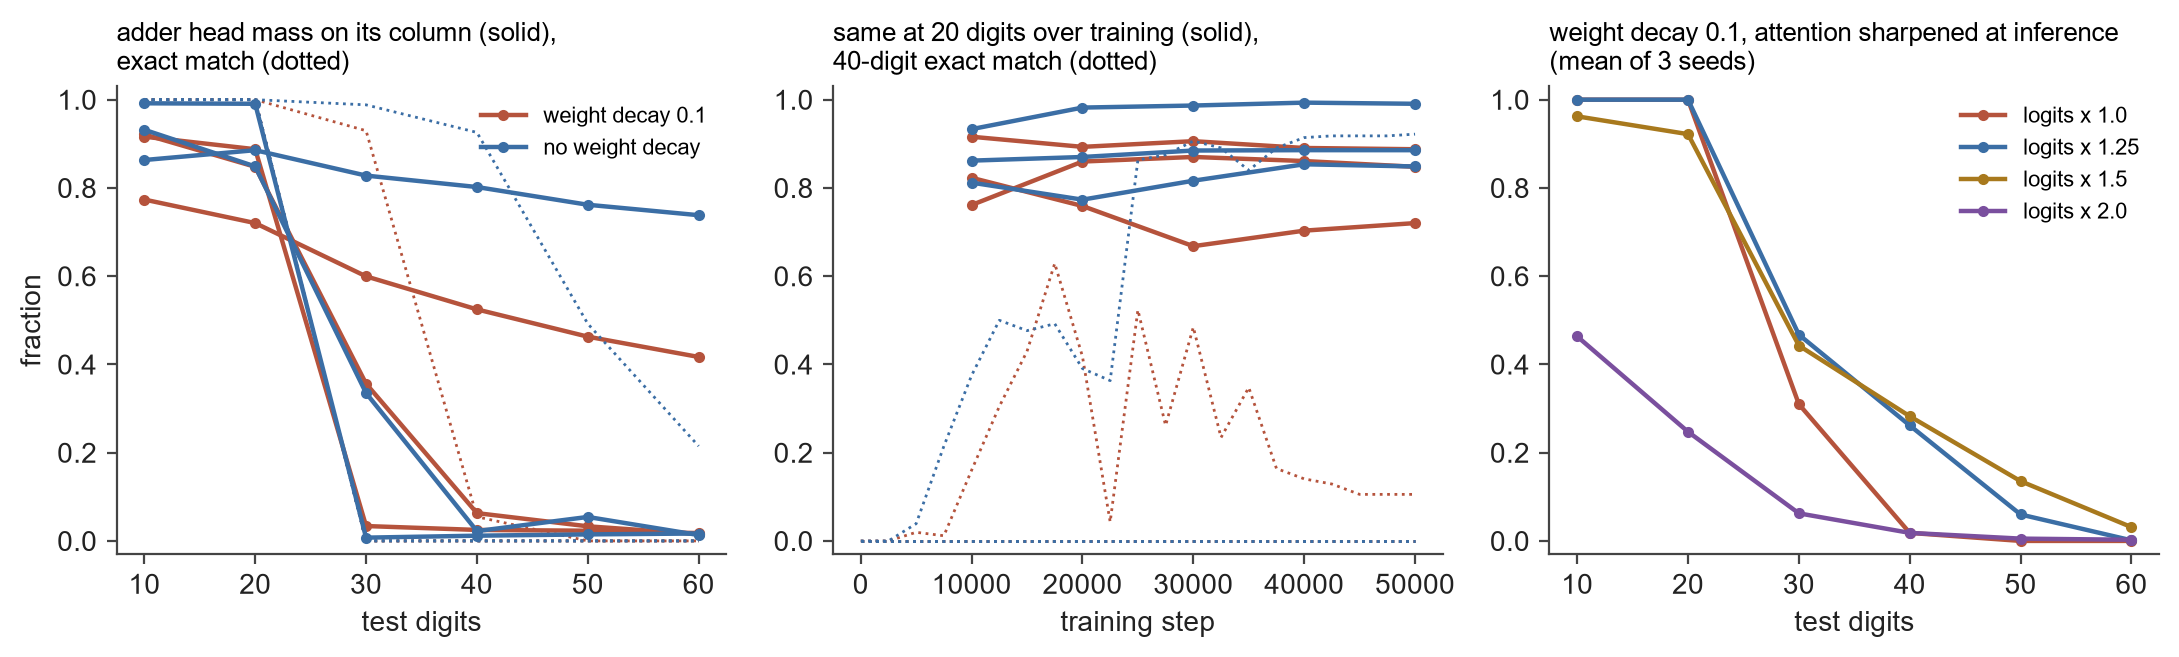
\includegraphics[width=\linewidth]{attention_dilution.png}
\caption{Left: the digit-adder head's attention mass on its column (solid) and exact match (dotted) versus test length, final checkpoints of six small position-coupling runs. Middle: the same mass at 20 digits during training, with 40-digit exact match. Right: exact match versus length when every head's logits are scaled at inference, mean of three seeds.}
\label{fig:dilution}
\end{figure}

\subsection{The intervention}

The intervention multiplies every head's attention logits by a constant $s$ before the softmax at inference; nothing is retrained. Table~\ref{tab:small} reports the small position-coupling seeds. Seed 0, whose 40-digit accuracy had declined from 63\% to 5\%, returns to 89\% at $s=1.4$ with in-distribution accuracy unchanged. Seed 1, which never reached 40 digits, rises from 0 to 46\% at 30. Seed 2, which never generalized, is unaffected at any $s$.

\begin{table}[t]
\centering
\begin{tabular}{llcccc}
\toprule
Seed & Logits $\times$ & 30 digits & 40 & 50 & 60 \\
\midrule
0 & 1.0 & 0.93 & 0.05 & 0 & 0 \\
0 & 1.4 & 1.00 & 0.89 & 0.34 & 0.04 \\
1 & 1.0 & 0 & 0 & 0 & 0 \\
1 & 1.4 & 0.46 & 0 & 0 & 0 \\
2 & any & 0 & 0 & 0 & 0 \\
\bottomrule
\end{tabular}
\caption{Exact match for the final checkpoints of the 3.4M position-coupling seeds (weight decay 0.1) with attention logits scaled at inference. Trained on 1 to 20 digits; 256 problems per length.}
\label{tab:small}
\end{table}

Figure~\ref{fig:sweep} and Table~\ref{tab:big} report the 11M model, trained on 1 to 30 digits and evaluated to 200. Seed 1 scores 69\% at 60 digits and 0\% at 80 and beyond as trained. At $s=2.0$ it scores 100\% exact match at every length from 10 to 200 digits on 128 problems per length: 6.7$\times$ the training length, matching the best factor reported for this method by \citet{cho2024position}, from a checkpoint that scored zero at 2.7$\times$. In-distribution accuracy is unchanged at $s=2.0$ and begins to fall at $s=2.5$. The other three seeds gain at 60 digits (from 0 to 84\%, 71\% and 65\%), gain nothing beyond 100 digits at any $s$, and are damaged by large $s$.

\begin{figure}[t]
\centering
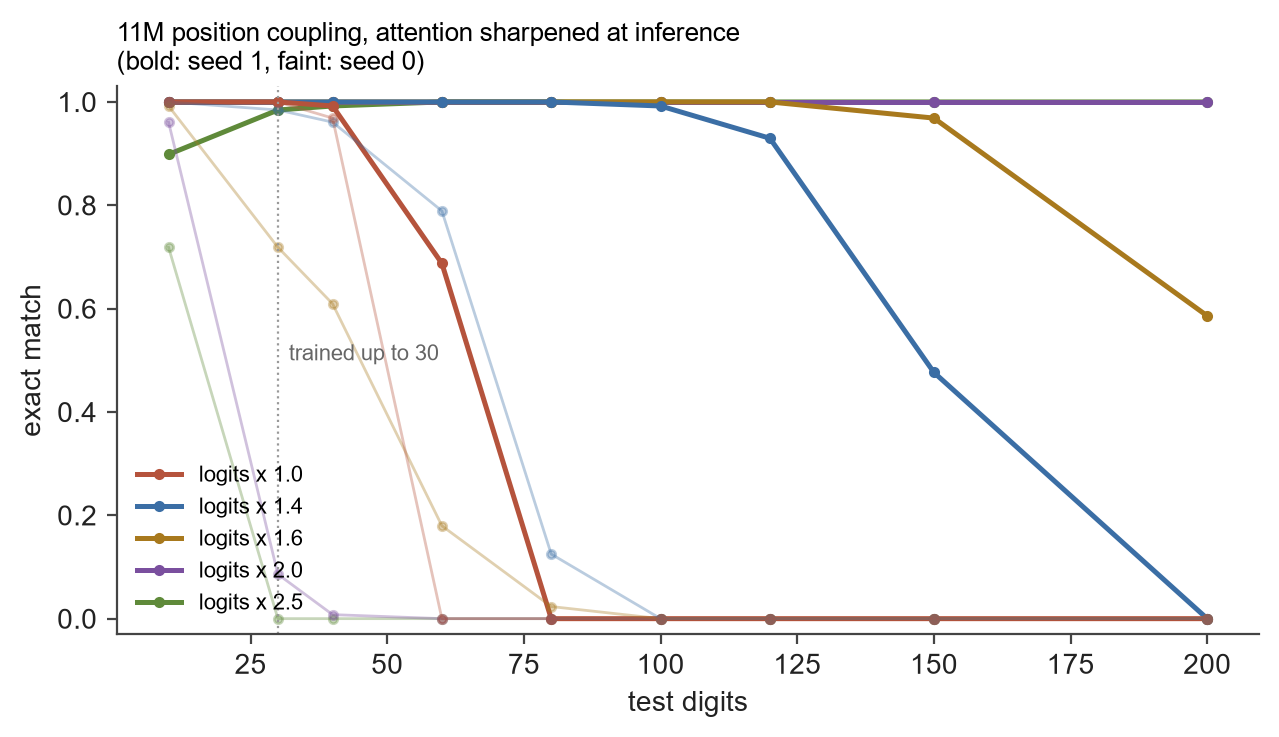
\includegraphics[width=0.85\linewidth]{sharpening_sweep.png}
\caption{Exact match versus test length for the four 11M position-coupling seeds with attention logits scaled at inference. Bold: seed 1; faint: the other seeds. Trained on 1 to 30 digits.}
\label{fig:sweep}
\end{figure}

\begin{table}[t]
\centering
\begin{tabular}{lcccccc}
\toprule
Logits $\times$ & 60 & 80 & 100 & 120 & 150 & 200 \\
\midrule
1.0 & 0.69 & 0 & 0 & 0 & 0 & 0 \\
1.4 & 1.00 & 1.00 & 0.99 & 0.93 & 0.48 & 0 \\
1.6 & 1.00 & 1.00 & 1.00 & 1.00 & 0.97 & 0.59 \\
2.0 & 1.00 & 1.00 & 1.00 & 1.00 & 1.00 & 1.00 \\
2.5 & 1.00 & 1.00 & 1.00 & 1.00 & 1.00 & 1.00 \\
\bottomrule
\end{tabular}
\caption{The 11M position-coupling model, seed 1, trained on up to 30 digits. Exact match on 128 problems per length. At $s=2.5$, accuracy at 10 digits falls to 0.90.}
\label{tab:big}
\end{table}

\subsection{Generality across runs}

Figure~\ref{fig:reach} applies the same sweep to every run in the study, at 2$\times$ and 3$\times$ each run's training length. Every position-coupling seed that generalized at any point during training gains; the one small abacus seed that generalized gains (70\% to 88\% at 40 digits, 0 to 55\% at 60); both large blankspace seeds gain at 40 digits (59\% and 63\% to 90\% and 86\%). No seed that never generalized gains at any $s$, in any method. The small blankspace models, whose sequence length is fixed by construction, are unaffected, consistent with the dilution account. The intervention thus does not add accuracy in general; it recovers a computation that training produced and left with insufficient attention contrast to execute at length.

\begin{figure}[p]
\centering
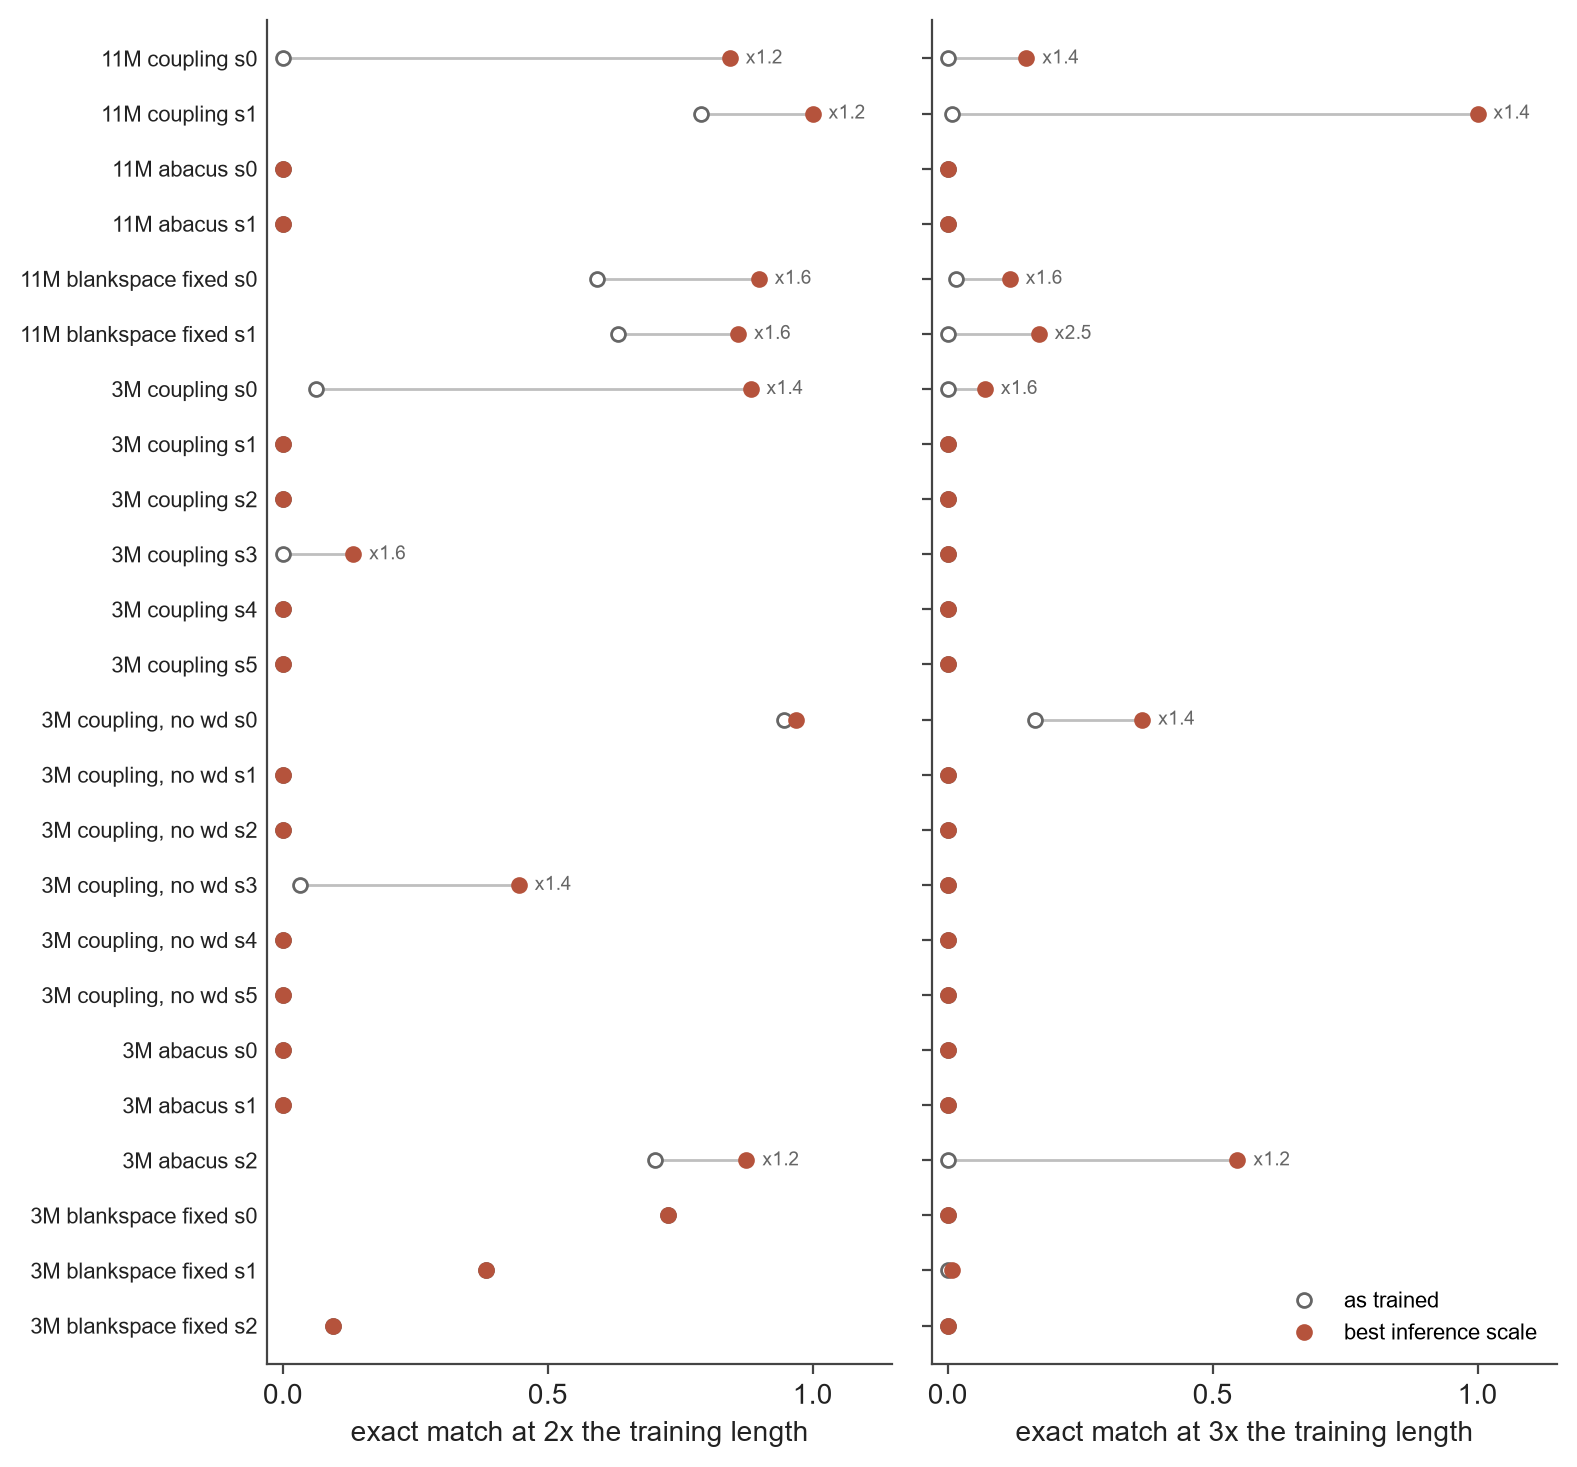
\includegraphics[width=0.95\linewidth]{sharpening_reach.png}
\caption{Exact match at 2$\times$ (left) and 3$\times$ (right) the training length for every run, as trained (open) and at the best inference scale (filled), which is marked when the gain is at least 5 points. Scales are chosen per run and length from $\{1, 1.2, 1.4, 1.6, 2, 2.5\}$ and applied on top of the scale the run was trained with (2 for rows marked ``trained x2'', 1 otherwise).}
\label{fig:reach}
\end{figure}

\subsection{Where the intervention acts}
\label{sec:layers}

Figure~\ref{fig:layers} scales the logits in subsets of layers of the 11M models. On seed 1, scaling layer 0 alone reproduces the full effect (100\% at 100 digits, 98\% at 150), scaling the first two layers is indistinguishable from scaling all six, and scaling every layer except layer 0 recovers nothing beyond the training length. Within layer 0, no single head is sufficient, and scaling heads H0, H3 or H5 alone reduces accuracy at 60 digits to near zero. The intervention thus acts on the joint attention pattern of the first layer. This is the layer that gathers the two operand digits of the current column from among all tokens sharing their position id, the lookup that a longer sequence dilutes, and it is where the digit-adder head of Section~\ref{sec:carry} is located in the small model. On seed 0 no subset of layers helps.

\begin{figure}[H]
\centering
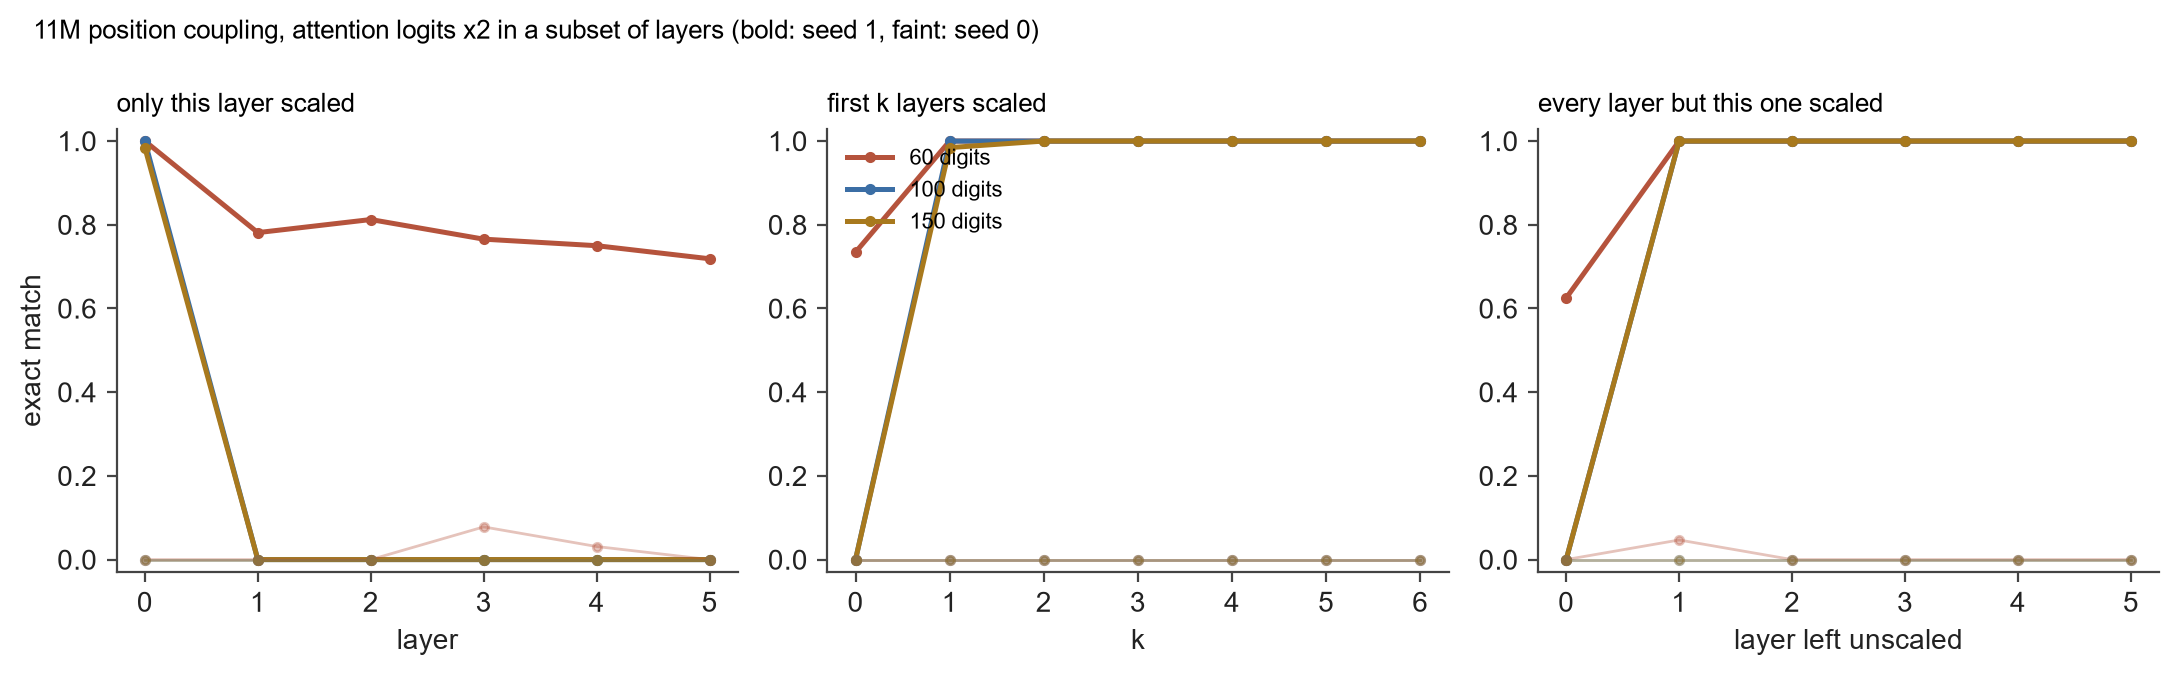
\includegraphics[width=\linewidth]{sharpen_by_head.png}
\caption{Exact match beyond the training length for the 11M position-coupling models when attention logits are scaled by 2 in a subset of layers. Left: one layer at a time. Middle: the first $k$ layers, with $k=0$ the trained model and $k=6$ all layers. Right: all layers except one. Bold: seed 1, which reaches 200 digits with all layers scaled; faint: seed 0.}
\label{fig:layers}
\end{figure}

\section{Training with an attention temperature}
\label{sec:training}

If insufficient contrast is the problem, a fixed temperature during training might prevent it. We trained position-coupling models with every head's logits multiplied by 2 throughout training: three small seeds and two large. On the small model this made generalization more reliable. All three seeds reach 85 to 100\% at 30 digits, where two of six ordinary seeds do, and two of three exceed 40\% at 40 digits, where one of six does. It did not prevent the decline (Figure~\ref{fig:erosion}, bottom row): the best small seed peaked at 91\% on 40 digits at step 10k and finished at 28\%, and one large seed peaked at 92\% on 60 digits at step 20k and finished at 4\%.

The two interventions stack, and training with the temperature changes which models the inference-time intervention helps. Applying a further factor of 1.4 to 1.6 on top of the trained temperature (Figure~\ref{fig:reach}, rows marked ``trained x2'') takes all five temperature-trained seeds from 4--41\% to 70--96\% at twice the training length, and the best large seed from 0 to 65\% at 100 digits. Every temperature-trained seed is recoverable in this sense, whereas among ordinarily trained seeds only the minority that generalized at some point are.

\section{Discussion}
\label{sec:discussion}

\paragraph{What the intervention shows.} The models that recover are the models that had the circuit. On the seed that reaches 200 digits, the entire effect is produced by sharpening the first layer, which performs the one lookup whose difficulty grows with sequence length under position coupling. The simplest reading is that training produces a correct algorithm whose first-layer attention is calibrated for the training lengths and is too diffuse at longer ones, and that the algorithm downstream of that lookup is length-invariant, as the carry analysis suggests it should be. Seeds that do not recover presumably lack a length-invariant circuit downstream, but we have not established what differs.

\paragraph{What it does not explain.} The decline during training is not accounted for. It survives a constant learning rate and a constant attention temperature, is only partly affected by weight decay, and does not appear as a loss of first-layer sharpness at the training length (Figure~\ref{fig:dilution}, middle). Yet the inference-time intervention recovers most of what the decline removed, so what is lost is recoverable by sharpening. One possibility is that the loss of contrast is specific to longer sequences and invisible at the training length; another is that a later part of the circuit degrades and is compensated by sharper first-layer attention. Distinguishing these requires tracking the full circuit across checkpoints and lengths.

\paragraph{Consequences for evaluation.} Two of our findings bear on how length generalization results are read. Reported numbers depend on the checkpoint, by up to 50 points here, and on an attention temperature that is rarely treated as a hyperparameter. A method's reported reach may reflect either.

\section{Limitations}

The 200-digit result is one seed of four; the other three gain from the intervention at twice the training length and no further. All experiments use models under 11M parameters, one task, and at most six seeds per configuration, on a single GPU. The relative-position control uses a per-head distance bias rather than the relative embeddings of \citet{shaw2018self}, and the headline combination of that submission \citep{aba2025} did not train under it, so our blankspace results are for its learned-position variant only. The sharpening factor is a constant chosen after training by sweeping; a length-dependent schedule in the spirit of \citet{chiang2022overcoming}, or a learned per-head temperature, was not tested.

\section{Conclusion}

On multi-digit addition, small transformers often learn a correct, length-invariant algorithm whose execution at longer lengths fails for lack of attention contrast in a single layer, and this contrast can be restored after training by scaling the attention logits. The same intervention distinguishes models that learned the algorithm from those that did not, and the accuracy it recovers is in many cases accuracy the model had earlier in training and lost. We release the code, all 53 trained checkpoints, and the scripts that produce every figure.

\subsubsection*{Acknowledgments and disclosure}
The code and the text of this paper were written with substantial assistance from Claude (Anthropic). The author designed the experiments, ran them, reviewed the code and the analysis, and is responsible for all claims. Code and configurations are at \url{https://github.com/Supergoatscriptguy/carrybit}; checkpoints are at \url{https://huggingface.co/SuperGoatScriptGuy/carrybit}.

\bibliographystyle{plainnat}
\bibliography{references}

\appendix

\section{Hyperparameters}
\label{app:hyper}

\begin{table}[h]
\centering
\begin{tabular}{lcc}
\toprule
 & Small & Large \\
\midrule
Layers & 4 & 6 \\
Width & 256 & 384 \\
Heads & 4 & 6 \\
MLP width & 1024 & 1536 \\
Parameters & 3.4M & 11M \\
Training operand digits & 1--20 & 1--30 \\
Steps & 50,000 & 60,000 \\
Batch size & 256 & 384 \\
Learning rate & $3\times10^{-4}$ & $2\times10^{-4}$ \\
Warmup steps & 1,000 & 2,000 \\
Schedule & cosine to 0 & cosine to 0 \\
Weight decay & 0.1 & 0.1 \\
Precision & bfloat16 autocast & bfloat16 autocast \\
Random position offset (abacus, coupling) & $U[0, 100]$ & $U[0, 200]$ \\
Test problems per length & 256 & 256 (128 for sweeps) \\
\bottomrule
\end{tabular}
\caption{Training configuration. Normalization is pre-LayerNorm; activations are ReLU; no dropout. The fixed-width blankspace models use 121 slots per number and, at the large scale, are trained on 1 to 20 digits with batch size 256 for 50k steps at learning rate $3\times10^{-4}$.}
\end{table}

\section{Per-seed results for the ladder}

\begin{table}[h]
\centering
\begin{tabular}{lcccc}
\toprule
Format & 20 digits & 30 & 40 & 50 \\
\midrule
Plain & 0.89 & 0 & 0 & 0 \\
Reversed & 1.00 & 0 & 0 & 0 \\
Reversed + zero pad & 1.00 & 0 & 0 & 0 \\
Zero pad + relative bias & 1.00 & 0 & 0 & 0 \\
Abacus & 1.00 & 0.31 (0.93) & 0.25 (0.75) & 0.08 (0.25) \\
Position coupling & 1.00 & 0.31 (0.92) & 0.04 (0.11) & 0 \\
Blankspace, variable width & 1.00 & 0 & 0 & 0 \\
Blankspace, fixed width & 0.99 & 0.81 (0.96) & 0.39 (0.68) & 0.04 (0.09) \\
Blankspace, fixed + relative bias & 0 & 0 & 0 & 0 \\
\bottomrule
\end{tabular}
\caption{Final-checkpoint exact match on the 3.4M model, mean over three seeds with the best seed in parentheses where seeds differ.}
\end{table}

\end{document}
